

\usetikzlibrary{shapes,arrows}
\usetikzlibrary{decorations.pathreplacing}


% Define block styles
\tikzstyle{decision} = [diamond, draw, fill=blue!20, 
    text width=4.5em, text badly centered, node distance=3cm, inner sep=0pt]

\tikzstyle{block} = [rectangle, draw, fill=gray!20, 
    text width=7em, text centered, minimum height=3em]

\tikzstyle{line} = [draw, -latex']

\tikzstyle{cloud} = [draw, ellipse,fill=red!20, node distance=3cm,
    minimum height=2em]

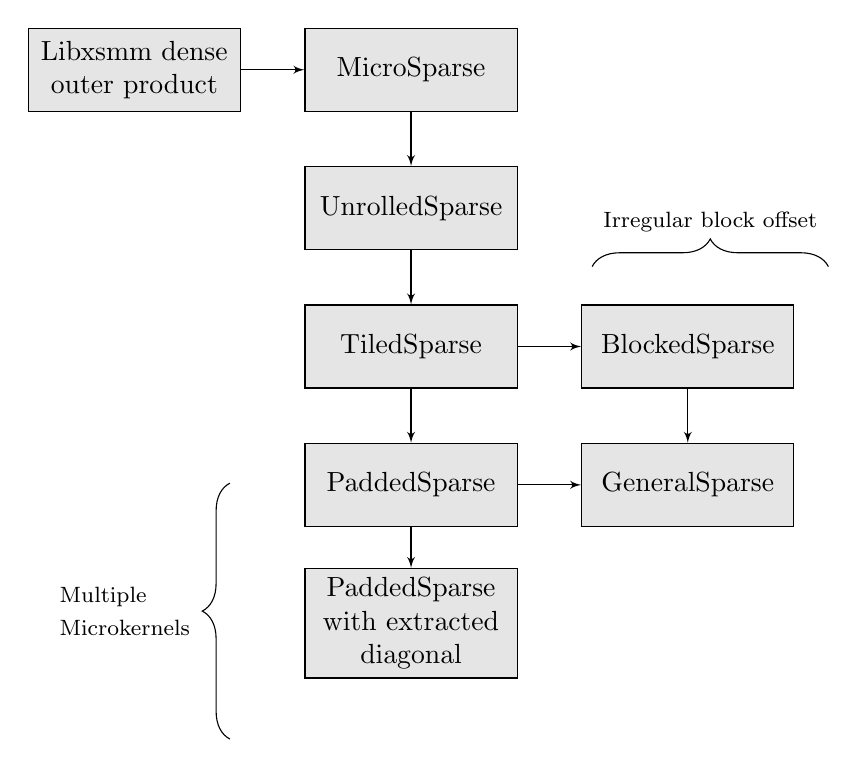
\begin{tikzpicture}[node distance = 5em, auto]
    % Place nodes

    \node [block] (microkernel) {MicroSparse};
    \node [block, left of=microkernel, node distance=10em] (libxsmm) {Libxsmm dense outer product};
    \node [block, below of=microkernel] (macrokernel) {UnrolledSparse};
    \node [block, below of=macrokernel] (tiledsparse) {TiledSparse};
    \node [block, right of=tiledsparse, node distance=10em] (blocksparse) {BlockedSparse};
    \node [block, below of=tiledsparse] (paddedsparse) {PaddedSparse};
    \node [block, below of=blocksparse] (generalsparse) {GeneralSparse};
    \node [block, below of=paddedsparse] (paddeddiagsparse) {PaddedSparse with extracted diagonal};

    %\node [block, left of=evaluate, node distance=3cm] (update) {update model};
    %\node [decision, below of=evaluate] (decide) {is best candidate better?};
    %\node [block, below of=decide, node distance=3cm] (stop) {stop};

    % Draw edges
    \path [line] (libxsmm) -- (microkernel);
    \path [line] (microkernel) -- (macrokernel);
    \path [line] (macrokernel) -- (tiledsparse);
    \path [line] (tiledsparse) -- (blocksparse);
    \path [line] (tiledsparse) -- (paddedsparse);
    \path [line] (paddedsparse) -- (generalsparse);
    \path [line] (blocksparse) -- (generalsparse);
    \path [line] (paddedsparse) -- (paddeddiagsparse);

    \draw [decorate,decoration={brace,amplitude=10pt},xshift=0pt,yshift=0pt]
(2.3,-2.5) -- (5.3,-2.5)node [black,midway,yshift=9pt] {\footnotesize Irregular block offset};

    \draw [decorate,decoration={brace,amplitude=10pt},xshift=0pt,yshift=0pt]
(-2.3,-8.5) -- (-2.3,-5.25) node [black,midway,xshift=-8pt,text width=5em] {\footnotesize Multiple\\ Microkernels};
    %\path [line] (evaluate) -- (decide);
    %\path [line] (decide) -| node [near start] {yes} (update);
    %\path [line] (update) |- (identify);
    %\path [line] (decide) -- node {no}(stop);
    %\path [line,dashed] (expert) -- (init);
    %\path [line,dashed] (system) -- (init);
    %\path [line,dashed] (system) |- (evaluate);
\end{tikzpicture}


